\chapter{Summary and beyond}

\section{Summary}
Finally, we have come to the end of this book. We started the book by introducing the most fundamental knowledge on modern radar technologies, establishing the technical background of Mode~S and ADS-B signals, and describing the hardware and software for receiving these signals. By the end of Part 1, I demonstrated how to set up a basic system, including the antenna, software-defined radio, and software tools. One thing worth noting is that I only illustrated the process of setting up two open-source tools under a Linux operation system, but they can certainly be used under other different operating systems.

The main focus of the book (Parts 2 and 3) has been to explain the detailed structures of all ADS-B and common Mode~S downlink messages, as well as to illustrate the decoding process with step-by-step examples when necessary. I tried to cover as many fields as possible in these messages. However, there may be certain fields that lack detailed explanation. The ICAO Annex Volume IV and ICAO Doc 9871 are always two excellent sources to find out more information on Mode S related topics.

In Part 2, we first introduced the basics of ADS-B, such as message structure, types, and different ADS-B versions. We then explained the structures and decoding processes for all ADS-B messages, including identification and category, airborne position, surface position, airborne velocity, and aircraft operation status. We also talked about parameters like uncertainties, accuracies, and integrities of ADS-B positions and velocities. Finally, in Part 2, we described the error control mechanism of ADS-B messages, which can be used to detect corrupt messages and with potential to correct them.

In Part 3, we focused on the decoding of other types of Mode~S messages. After explaining the basics of Mode~S, we discussed all-call replies, surveillance replies, ACAS messages, and Comm-B messages. These are messages transmitted in different Mode~S downlink formats, with Comm-B downlink containing the most information. In theory, it supports up to 256 message types (not all are used currently). Within Comm-B communication, some subsets of messages are commonly used by air traffic controllers. Then, we continued with the decoding of nine message types in three groups of Mode~S services, which are Mode~S elementary surveillance, Mode~S enhanced surveillance, and Mode~S meteorological services. As the third party receiver, the difficulty of decoding Comm-B messages is that we can not easily identify the types of messages like ADS-B messages. So, in the last chapter of this part, we discussed the important aspect of how to infer Comm-B types from downlink messages.


\section{Crowd-sourced networks}

In chapter 2, we talked about the coverage of ADS-B receivers. Even with the perfect location, one receiver can only cover a maximum area of around 400 km radius, due to the curvature of the Earth. The coverage is further reduced when the antenna is not free of obstacles like buildings and mountains. 

To cover full flight trajectories for a larger area, a group of receivers needs to be deployed. Furthermore, to have coverage over the entire continent (or multiple continents), an even larger network of receivers is needed. To deploy and maintain receivers on such a larger scale is difficult for any individual entity. That is the reason for crowd-sourced ADS-B networks. 

A crowd-sourced network usually consists of a large group of enthusiasts who are voluntarily feeding their receiver data to a central server (or cluster of servers) on the internet owned by an entity. The owner of the service can be a commercial company or a non-profit organization. These companies often provide free premium user accounts to contributors in return for their data. Some companies also provide free receivers for users to host in areas with less coverage. In such cases, they often make agreements with receiver hosts to maintain and keep the receiver online as much as possible. In Table \ref{tb:adsb_networks}, several ADS-B networks are listed.

\begin{table}[ht]
\caption{A short list of ADS-B receiver networks}
\label{tb:adsb_networks}
\begin{threeparttable}
\begin{tabular}{|l|l|l|l|}
\hline
\textbf{Name} & \textbf{Type} & \textbf{Founded} & \textbf{Number of receivers} \\ \hline
FlightAware & Commercial & 2005 & 30,000\tnote{*} \\ \hline
FlightRadar24 & Commercial & 2006 & 25,000\tnote{*} \\ \hline
RadarBox24 & Commercial & 2007 & unknown \\ \hline
OpenSky network & Non-profit / research & 2013 & 3,400\tnote{*} \\ \hline
ADS-B Exchange & Non-profit & 2016 & unknown \\ \hline
\end{tabular}
\begin{tablenotes}
\item[*] Number of receivers obtained from each company's website, as of October 2020.
\end{tablenotes}
\end{threeparttable}    
\end{table}

Another advantage of having a network of receivers is that it can be used to locate aircraft or validate their locations using multilateration \cite{kaune2012}, and this capability can be applied to any Mode A/C/S signals transmitted by aircraft. This technique has been used by many receiver networks. It is specifically useful to locate aircraft that are not equipped with ADS-B compliant transponders.

{\large\textbf{OpenSky network}}

Among these crowd-sourced networks, the OpenSky network \footnote{https://opensky-network.org} is one of the most well-known research networks in the air transportation research community. It is a crowd-sourced network that includes volunteers and researchers around the world. Currently, it has good coverage over Europe and a large part of North America. In Figure \ref{fig:opensky_coverage}, we can see the current global coverage of the OpenSky network.

\begin{figure}[ht]
    \centering
    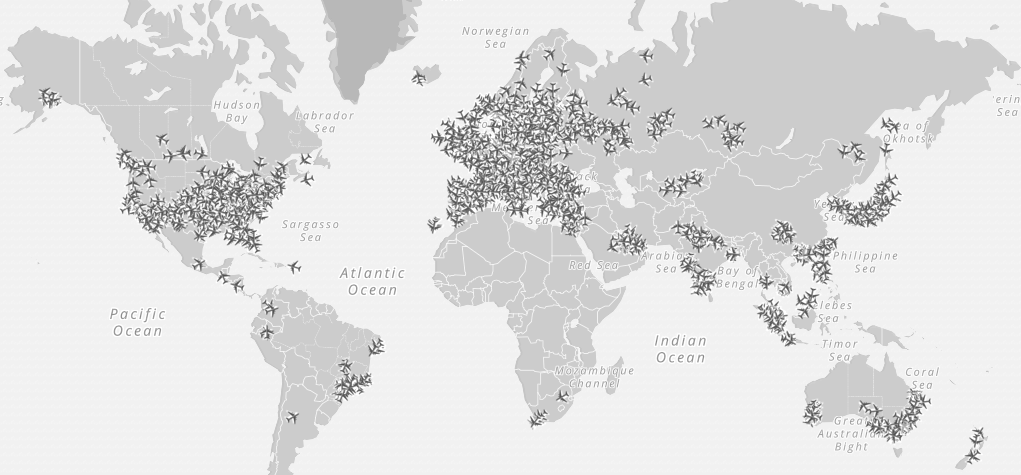
\includegraphics[width=\columnwidth]{figures/conclusion/opensky.png}
    \caption{Coverage of OpenSky network, as of November 2020}
    \label{fig:opensky_coverage}
\end{figure}

The OpenSky network provides users free and unlimited access to its data for non-commercial usages \cite{schafer2014opensky}. It is possible to access its live ADS-B traffic data through web APIs. Access to historical data is also possible through its Impala shell. However, the user must request this permission first. I also wrote a Python library,\footnote{https://github.com/junzis/pyopensky} which facilitates the access and decoding of raw Mode~S messages from the OpenSky historical database using its Impala interface \cite{sun2019pyopensky}. Another tool, \emph{traffic}, can also be used to access the OpenSky historical database \cite{olive2019}.

If you are setting up a receiver or have an existing receiver, I strongly encourage you to consider sharing your Mode~S feed with the OpenSky network to increase coverage and to support open flight data for researchers. Guides on how to feed data to OpenSky can be found on its website.\footnote{https://opensky-network.org/contribute/improve-coverage}

\section{Additional data}

For many air traffic-related studies, we frequently require information that is not transmitted in ADS-B and Mode~S. One of the first things we often need is an aircraft database that can map the transponder address from ADS-B or Mode~S to aircraft registration and aircraft type. 

A few countries, including the United States, make this information publicly available for download. However, a large part of this information is not officially available or behind paywalls. There are many different sources of aircraft data that are maintained by hobbyists and volunteers on the internet. One of the most comprehensive databases for aircraft is also maintained by OpenSky network. A select list of data sources can be found on the \emph{Open Aviation Data} website.\footnote{https://atmdata.github.io/sources/}.

On this website, a few other common data sources are also listed, including, for example, aircraft performance database, engine emission data, and weather data. All these data sources are available for public use.


\section{Congestion}
In the first chapter of this book, we discussed all types of signals that are transmitted over the 1090 megahertz frequency. They include Mode~A, Mode~C, and Mode~S. Due to the mix of different types of transponders from a wide range of aircraft including both commercial and general aviation, all these modes of surveillance are still in use nowadays. In addition to the increasing number of operational aircraft, the frequency congestion can be a quite serious issue during the daytime in busy airspace. 

In a recent study \cite{sun2020rf}, using a software defined radio receiver, we found that more than 60 \% of the ADS-B signals we received during the daytime are corrupted, within the airspace we are located. Figure \ref{fig:adsb_corruption} illustrates the severity of the frequency congestion during one day of radio frequency testing for Dutch airspace.

\begin{figure}[ht]
    \centering
    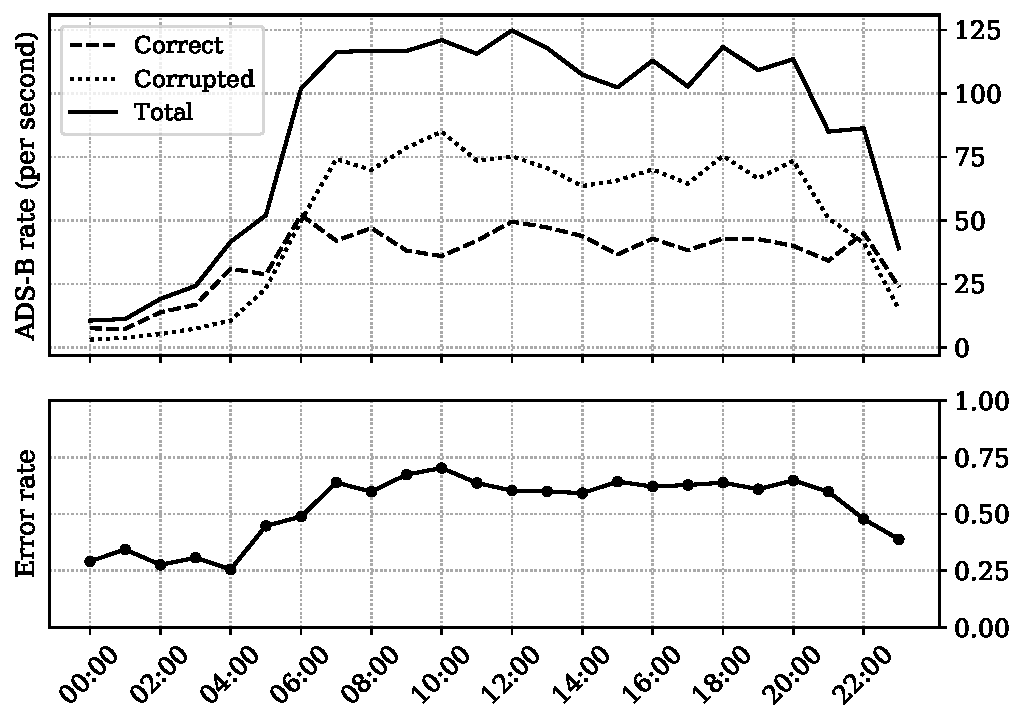
\includegraphics[width=0.7\columnwidth]{figures/conclusion/adsb_corruption.pdf}
    \caption{Corruption detected in ADS-B messages during a 24 hour period on 29
    January, 2020.}
    \label{fig:adsb_corruption}
\end{figure}

High congestion of the 1090 megahertz radio frequency applies for many busy airspaces. The situation is especially serious in Europe, where the air traffic density is quite high during daytime operations. The mix of all different modes of surveillance (A/C/S) combined with the continuously increasing air traffic makes the channel busier with time.  

\section{Future of Mode~S and ADS-B}
Reducing radio frequency congestion is one important area for future research. Some potential solutions to help us mitigate this problem in the future include, for example:

\begin{itemize}
    \item Reduce and phase out Mode~A and Mode~C surveillance.
    \item Balance Mode~S interrogations among different surveillance radars.
    \item Migrate interrogation based surveillance to broadcast (like ADS-B).
    \item Introduce more error resistance modulation and channel coding methods.
    \item Make use of alternative frequencies.
\end{itemize}

Another issue is the global coverage of ADS-B. Currently, it is still difficult to fully track aircraft over the oceans, due to the lack of ground stations. One trend is to make use of satellites for receiving and relaying ADS-B messages transmitted by planes to ground stations \cite{noschese2011}. Companies like Aireon and Spire are launching satellites that can receive ADS-B signals. 

It is still challenging for satellites to handle signals with a low signal to noise ratio given the high satellites orbits, as well as the high signal garbling rates caused by their large coverage. Furthermore, a large quantity of oceanic ADS-B data is located behind paywalls, which makes it hard for researchers to take advantage of space-based ADS-B data. 

To this end, how to help researchers access higher-quality open surveillance data over a larger geographic scope, is a question that remains for me, you, and the entire research community to answer.